\documentclass[12pt, a4paper, UTF8, openany]{ctexbook}

\usepackage{geometry}%设置页边距
\geometry{left=1.54cm, right=1.54cm, top=2.18cm, bottom=2.18cm}

\usepackage{tikz}%绘图
\usetikzlibrary{calc}%绘图时计算
\usetikzlibrary{angles}%角度标识
\usetikzlibrary{quotes}%标签

\usepackage{amsmath, amssymb}%数学

\usepackage{array}%表格基础设置
\usepackage{longtable}%跨页表格
\usepackage{booktabs}%表格水平线

\usepackage[colorlinks = true, 
            linkcolor = black]{hyperref}%超链接跳转

\usepackage{color}

\newcommand{\dif}{\mathrm{d}}
\newcommand{\sdif}{\,\mathrm{d}}

% \newcommand{\vect}[1]{\overrightarrow{#1}}
\newcommand{\vect}[1]{\mathbf{#1}}
\newcommand{\vecr}{\vect{r}}
\newcommand{\vecv}{\vect{v}}
\newcommand{\veca}{\vect{a}}
\newcommand{\vecat}{\vect{a_{t}}}
\newcommand{\vecan}{\vect{a_{n}}}
\newcommand{\vecf}{\vect{F}}
\newcommand{\vecalpha}{{\alpha}}%mathbf 对 alpha 无效
\newcommand{\et}{\vect{e_{t}}}
\newcommand{\en}{\vect{e_{n}}}
\newcommand{\vecp}{\vect{p}}
\newcommand{\vecm}{\vect{M}}
\newcommand{\vecl}{\vect{L}}

\newcommand{\cross}{\times}

\linespread{1.05}%行间距
\setlength{\parskip}{8pt}%段落间距
\setlength{\parindent}{0pt}%不缩进

\setcounter{chapter}{-1}

\title{Physics}
\author{K}

\begin{document}
    \maketitle

    \tableofcontents % use LaTeXmk
    \cleardoublepage % 正文从新页开始，利好双面打印

    \chapter{方法论}
    $\dif s = |\dif \vect{r}| \neq \dif |\vect{r}|$

    利用质心。

    时间元与空间元转换；孤立元与组合元转换。

    \chapter{力学}

    \section{运动学}
    $\vecr$: 位矢 \\
    $s$: 路程

    $\vecv = \dfrac{\dif \vecr}{\dif t}\quad$
    $v = |\vecv| = \dfrac{|\dif \vecr|}{\dif t} = \dfrac{\dif s}{\dif t}$

    $\veca = \dfrac{\dif \vecv}{\dif t}$
    
        \subsection{基本问题}
            知 $r$：导。

            知 $v/a$：积。
            \begin{itemize}
                \item $a = a(t)$ \\
                    积。
                \item $a = a(x)$: e.g. $F_{\text{引}}$ \\
                    $a(x) = \dfrac{\dif v}{\dif t} = \dfrac{\dif v}{\dif x} \cdot \dfrac{\dif x}{\dif t} 
                    = \dfrac{\dif v}{\dif x} \cdot v \implies v = v(x)$ \\
                    $v(x) = \dfrac{\dif x}{\dif t} \implies t = t(x) \implies x = t^{-1}(t)$
                \item $a = a(v)$: e.g. 风阻 \\
                    $a(v) = \dfrac{\dif v}{\dif t} \implies t = t(v) \implies v = t^{-1}(t)$ \\
                    $v = \dfrac{\dif x}{\dif t(v)} \implies x = x(v)$
            \end{itemize}

        \subsection{自然坐标系}
        $\et$: 切向 \\
        $\en$: 法向，指向曲线凹侧

        几何：$v = \rho\omega$，$\vecat = \rho\vecalpha$，$\dif s = \rho \theta$

        $\vecr = \vect{0}$，因以自身位置为原点。

        $\vecv = \dfrac{\dif \vecr}{\dif t} = \dfrac{\dif \vecr}{\dif s} \cdot \dfrac{\dif s}{\dif t} 
        = \dfrac{\dif \vecr}{\dif s} \cdot v = v \cdot \et$。
        速度总沿切线方向。

        $\begin{aligned}
            \veca &= \dfrac{\dif \vecv}{\dif t} = \dfrac{\dif (v \cdot \et)}{\dif t} 
            = \dfrac{\dif v}{\dif t} \cdot \et + \dfrac{\dif \et}{\dif t} \cdot v \\
            &= \dfrac{\dif v}{\dif t} \cdot \et + \dfrac{\dif (1 \cdot \theta)}{\dif t} \cdot \en \cdot v
            = \dfrac{\dif v}{\dif t}\cdot \et + v\omega \cdot \en = \vecat + \vecan
        \end{aligned}$ \\
        $\vecat = \rho\vecalpha$，其中 $\vecalpha = \dfrac{\dif \omega}{\dif t}$ 为角加速度，和 $\et$ 同向。\\
        $\vecan = v\omega \cdot \en = \dfrac{v^2}{\rho} \cdot \en = \rho^2\omega \cdot \en$

        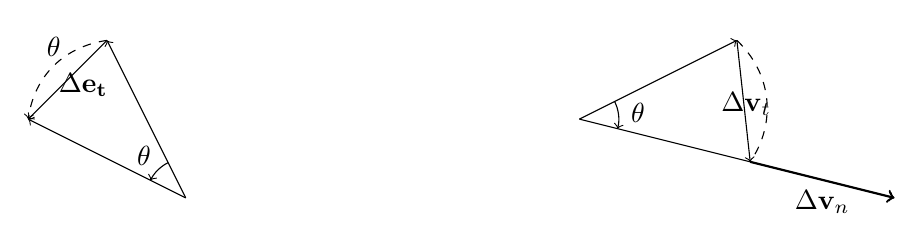
\begin{tikzpicture}
            \coordinate (a) at (0, 0);
            \coordinate (b) at (-1, 2);
            \coordinate (c) at (-2, 1);

            \draw [->] (a) -- (b);
            \draw [->] (a) -- (c);
            \draw [->] (b) -- node[below, pos = 0.3]{$\Delta \et$} (c);
            \draw [->, dashed] (b) to[bend right = 36.87] node[above, midway]{$\theta$} (c);

            \draw pic[->, draw = black, "$\theta$", angle eccentricity = 1.5] {angle = b--a--c};

            \coordinate (x) at (5, 1);
            \coordinate (y) at (7, 2);
            \coordinate (z) at (9, 0);
            \coordinate (w) at ($(5, 1)!sqrt(5)/sqrt(17)!(9, 0)$);

            \draw [->] (x) -- (y);
            \draw [->] (x) -- (z);
            \draw [->] (y) -- node[above, pos = 0.7]{$\Delta \vect{v}_{t}$} (w);
            \draw [->, thick] (w.south) -- node[below, midway]{$\Delta \vect{v}_{n}$} (z.south);
            \draw [-, dashed] (y) to[bend left = 40.5] (w);

            \draw pic[<-, draw = black, "$\theta$", angle eccentricity = 1.5] {angle = z--x--y};
        \end{tikzpicture}

    \section{动力学}
        \subsection{牛顿定律}
        力 $F := \dfrac{\dif \vect{p}}{\dif t} = \dfrac{\dif (m\vecv)}{\dif t}$
        
        \begin{itemize}
            \item 牛一：$F = 0$，$\vecv = \text{Const vector}$
            \item 牛二：$v << c$ 时，$F = m\veca$
            \item 牛三：$F = -F'$
        \end{itemize}

        \subsection{相对性原理}
        惯性系：使牛顿定律成立的参考系。\\
        非惯性系：牛顿定律不成立，补充惯性力也是基于惯性系而言。所有分析必须基于惯性系。

        相对惯性系匀速运动的参考系仍为惯性系：$\vecv = \vecv' + \vect{u} \implies \veca = \veca' \implies F = F'$ \\
        力学相对性原理：在惯性系内做实验，无法判断自身是否在运动。

        \subsection{换系}
        $\vecr_{PO} = \vecr_{PO'} + \vecr_{O'O} \; \implies \; 
        \dfrac{\vecr_{PO}}{\dif t} = \dfrac{\vecr_{PO'}}{\dif t} + \dfrac{\vecr_{O'O}}{\dif t} \; \implies \;
        \vecv_{PO} = \vecv_{PO'} + \vecv_{O'O}$

        （物体对系）绝对速度，为（物体对另一系）相对速度与（另一系对系）跟随速度之和。与是否处于惯性系无关。

        同理，$\veca_{PO} = \veca_{PO'} + \veca_{O'O}$

        若 O 为惯性系，在 O 系下做受力分析并分别讨论 PO'/O'O 方向的运动。本质是运动的分解，即使 O' 不为惯性系亦可。

        {\heiti 动能/动量均与参考系选取相关}。

    \section{能量}
    元功 $\dif W = F \cdot \dif\vecr = F \cos\theta |\dif r| = F \cos\theta \sdif s$。
    力在距离上的累积，代数和。向量点乘保证了功可以正交分解，变为在各坐标轴上的分量和。

    功率 $P = \frac{\dif W}{\dif t} = F \cdot \vecv$

        \subsection{动能}
        $F \cdot \dif\vecr = m \frac{\dif\vecv}{\dif t} \cdot \dif\vecr 
        = m \sdif\vecv \cdot \frac{\dif\vecr}{\dif t} = m \sdif\vecv \cdot \vecv$。
        其中向量数乘对向量点乘分配。在 $\Delta t \to 0$ 下，$\vecv_{t}$ 与 $\vecv_{t + \Delta t}$ 近乎共线，
        亦即 $\vecv$ 与 $\dif\vecv$ 近乎共线。$\implies m \sdif\vecv \cdot \vecv = mv\sdif v$ \\
        $W = \int_{a}^{b} \dif W = \int_{a}^{b} mv\sdif v = \frac{1}{2}mv^2|_{a}^{b}$

        动能 $E_{k} := \frac{1}{2}mv^2$ \\
        动能定理：$W = \Delta E_{k}$

        特别地，{\heiti 动能可以正交分解}。$E_{k} = \sum \frac{1}{2} m v_{i}^2$。

        \subsection{机械能}
        保守力：$\vect{F}(\vect{r}) = f(r)\vecr$。力（或反向延长线）指向定点，大小仅与 $r$ 相关。\\
        势能 $E_{p}$，力 $F = {\color{red}-} \nabla E_{p}$。一般取无穷远处为零势能面。\\
        做功 $W_{1 \to 2} = {\color{red}-} \Delta E_p = E_{p1} - E_{p2}$，与路径无关。

        \begin{itemize}
            \item 引力 \\
                $\dif W = -G \frac{mM}{r^2} \vect{e}_r \cdot \dif\vecr$。
                如法炮制，$\vect{e}_r$ 与 $\dif\vecr$ 共线 $\implies \vect{e}_r \cdot \dif\vecr = \dif r$。\\
                $W = \int_{r_1}^{r_2} -G\frac{mM}{r^2}\sdif r = GmM(\frac{1}{r_2} = \frac{1}{r_1})$
            \item 弹簧 \\
                $W = -\frac{1}{2}k (x_2^2 - x_1^2)$
        \end{itemize}

        \subsection{质点系}
        $\dif W = \dif W_{\text{外}} + \dif W_{\text{内}}$。故不受外力不代表系统做功。

        特别地，一对相互作用力的总功：\\
        $\begin{aligned}
            \dif W &= F_{2 \to 1} \cdot \dif\vecr_1 + F'_{1 \to 2} \cdot \dif\vecr_2 
            = F_{2 \to 1} \cdot \dif\vecr_1 - F_{1 \to 2} \cdot \dif\vecr_2 
            = F_{2 \to 1} \cdot \dif(\vecr_1 - \vecr_2) \\
            &= F_{2 \to 1} \cdot \dif\vecr_{2 \to 1}
        \end{aligned}$ \\
        以一个物体为参考，则总功为 $F$ 在该系下对另一物体做的功。
        尽管单个力的功与参考系选取有关，但一对相互作用力的总功与参考系无关。\\
        推论：{\heiti 摩擦力总功恒负}。

        无外力做功，无非保守内力做功，则机械能守恒。

    \section{动量}
    冲量 $I = \int F \sdif t$。力在时间上的累积，矢量和。

    $F = \frac{\dif p}{\dif t} \implies I = \int F \sdif t = \int \dif p = \Delta p = m \Delta v$ \\
    动量定理：$I = \Delta p$

        \subsection{质点系}
        质点系：$\sum I_{\text{内}} = \sum F\sdif t + F'\sdif t = 0$，$I = I_{\text{外}} + I_{\text{内}} = I_{\text{外}}$

        外力为零时，系统动量守恒。

        \subsection{质心表述}
        $\vecp = \sum m_i \vecv_i = \sum m_i \frac{\dif \vecr_i}{\dif t} 
        = \frac{\dif}{\dif t} (\sum m_i \vecr_i) = \frac{\dif}{\dif t} M (\sum \frac{m_i}{M} \vecr_i) = M \vecv_{c}$

        进一步地，$\vecv_{c} = \frac{\vecp}{M} = \frac{\sum m_i \vecv_i}{M}$

        $F_{\text{外}} = \frac{\dif p}{\dif t} = \frac{\dif p_{c}}{\dif t} = m a_c$

        {\heiti 质心的位矢和速度均为重量的带权重心}。
        系统总动量，等于质心动量。外力也可视为作用于这一质点。

    \section{转动}
    各物理量均对某一参考点/旋转轴而言，不能脱离参考。

    对偶：
    \begin{longtable}[h]{l l | l l}
        位移/速度/加速度 & $\vecr/\vecv/\veca$ & 
        角度/角速度/角加速度 & $\vect{\theta}/\vect{\omega}/\vect{\alpha}$ \\
        \addlinespace

        质量 & $m$ & 转动惯量 & $J$ \\
        \addlinespace

        力 & $\vecf = m \veca = \frac{\dif \vecp}{\dif t}$ & 
        力矩 & $\vecm = J \alpha = \frac{\dif \vecl}{\dif t}$ \\
        \addlinespace

        元功/动能 & $\begin{matrix} \dif W &= \vecf\cdot\dif\vecr \\ E_k &= \frac{1}{2}m \vecv^2 \end{matrix}$ & 
        元功/转动动能 & $\begin{matrix} \dif W &= \vecm\cdot\dif\theta \\ E_k &= \frac{1}{2}J\omega^2 \end{matrix}$ \\
        \addlinespace

        动量 & $\vecp = m \vecv$ & 角动量 & $\vecl = J \omega$
    \end{longtable}

        \subsection{运动学}
        角度逆正顺负，服从右手螺旋定则。由此定义矢量 $\theta$，$\omega$，$\alpha$。

        $\vecv = \vecr \cross \omega$

        \subsection{动力学}
        力矩 $\vecm = \vecr \cross F = Fr\sin\theta$。\\
        单位 N$\cdot$m，量纲同焦耳。

        下讨论定轴转动，即各部分 $\omega/\alpha$ 永远相同。

        对刚体，各部分无相对移动，相互作用力作用点重合，力臂相同。$\implies M + M' = 0 \implies M_{\text{内}} = 0$

        对刚体，仅需考虑外力，考虑切向分力 $F_{it}$，
        $F_{it} = m_i\vecat = m_i r_i \alpha \implies F_{it} r_i = m_i r_i^2 \alpha 
        \implies r_i \cross F_i = m_i r_i^2 \alpha$ \\
        $\implies \sum r_i \cross F_i = (\sum m_i r_i^2) \alpha$

        转动惯量：$J = \sum m_i r_i^2$，任意刚体需积分/实验。\\
        转动定律：$M = J \alpha$，与牛二对偶。

        特别地，{\heiti 转动惯量可以正交分解}。$J = \sum J_i$

        \subsection{能量}
        $\dif W = F \cdot \dif \vecr = F_{t} s = F_{t} r \sdif\theta \implies \dif W = \vecm \cdot \sdif\theta$ \\
        $P = \frac{\dif W}{\dif t} = \vecm \cdot \omega$ \\
        $M/\theta/\omega$ 均为矢量，均为点乘。

        $E_{k} = \sum \frac{1}{2} m_i v_i^2 = \sum \frac{1}{2} m_i r_i^2 \omega^2 
        = \frac{1}{2}(\sum m_i c_i^2)\omega^2$

        转动动能 $E_{k} = \frac{1}{2} J \omega^2$ \\
        转动的动能定理 $W = \Delta E_{k}$

        \subsection{角动量}
        角动量 $\vecl = \vecr \cross \vecp = \vecr \cross m\vecv$；$\vecl = J\omega$

        $\vecm = \vecr \cross F = \vecr \cross \frac{\dif (m\vecv)}{\dif t} 
        = m \vecr \cross \frac{\dif \vecv}{\dif t}$ \\
        而 $\frac{\dif}{\dif t}(\vecr \cross \vecv) = \frac{\dif \vecr}{\dif t} \cross \vecv + 
        \vecr \cross \frac{\dif \vecv}{\dif t} = \vecv \cross \vecv + \vecr \cross \frac{\dif \vecv}{\dif t} 
        = \vecr \cross \frac{\dif \vecv}{\dif t}$ \\
        $\implies \vecm = \frac{\dif}{\dif t} (\vecr \cross m\vecv)$

        角动量定理：$\vecm = \frac{\dif \vecl}{\dif t} = \frac{\dif}{\dif t} (\vecr \cross m\vecv)$ \\
        冲量距：$\vecm \sdif t = \dif \vecl$

        对刚体，$L = \sum m_i \vecr_i \cross \vecv_i = \sum m_i \vecr_i \cross (\vecr_i \cross \omega) 
        = \sum m_i r_i^2 \omega = J\omega$

        角动量守恒：$\vecm = \vect{0}$ 时，$\vecl = \text{Const vector}$。这不代表 $F = \vect{0}$。\\
        {\heiti 应用}：开普勒第二定律

        \subsection{质心表述}
        平行轴定理：记刚体绕通过质心的轴线旋转时，转动惯量为 $J_c$，则绕平行与该轴的轴旋转时转动惯量 $J = J_c + Md^2$，
        其中 $d$ 为两轴线的距离。\\
        证：$J$ 可正交分解，考虑 $x$ 轴分量，记 $d$ 在 $x$ 的投影为 $x_0$。不妨令质心 $x_c = 0$，则 $\sum m_i x_i = 0$。
        $J = \sum m_i (x_i - x_0)^2 = (\sum m_i x_i^2) + (\sum m_i) x_0^2 - 2x_0(\sum m_i x_i) = J_c + Mx_0^2$。

        $\begin{aligned}
            \vecl &= \sum \vecr_i \cross m_i \vecv_i = \sum (\vecr_c + \vecr_{i \to c}) \cross m_i \vecv_i 
            = \vecr_c \cross (\sum m_i \vecv_i) + \sum \vecr_{i \to c} \cross m_i (\vecv_c + \vecv_{i \to c}) \\
            &= \vecr_c \cross M\vecr_c + (\sum m_i \vecr_{i \to c}) \cross \vecv_c 
            + \sum \vecr_{i \to c} \cross m_i \vecv_{i \to c} \\
            &= \vecr_c \cross M\vecr_c + \vecr_{c \to c} \cross \vecv_c + \sum \vecr_{i \to c} \cross m_i \vecv_{i \to c} 
            = \vecr_c \cross M\vecr_c + \sum \vecr_{i \to c} \cross m_i \vecv_{i \to c}
        \end{aligned}$ \\
        质点系总角动量，可分解为质心角动量与各点相对质心的角动量。\\
        $\vecl = \vecl_{\text{轨道}} + \vecl_{\text{自旋}}$：
        $\vecl_{\text{轨道}} = \vecr_c \cross M \vecr_c$；
        $\vecl_{\text{自旋}} = \sum \vecr_{i \to c} \cross m_i \vecv_{i \to c}$

        $E_{k} = \sum \frac{1}{2} m_i \vecv_i^2 = \sum \frac{1}{2} m_i (\vecv_{i \to c} + \vecv_c)^2 
        = \frac{1}{2} (\sum m_i) \vecv_c^2 + (\sum \frac{1}{2} m_i \vecv_{i \to c}^2) 
        + (\sum m_i \vecv_{i \to c}) \cdot \vecv_c$ \\
        以质心为参考系，则 $\vecv_c = \vect{0}$，又由 $\vecv_c$ 为带权重心知 $\sum m_c \vecv_{i \to c} = \vect{0}$。\\
        $\implies E_{k} = \frac{1}{2} M \vecv_c^2 + \frac{1}{2} J\omega^2$

        刚体无滑动滚动时，即运动可视为质心的平动与各点绕质心转动之和，则总动能为质心动能与转动动能之和。

\end{document}